%=========================================================================

\chapter{Úvod}
Tento manuál je dokumentáciou k~projektu z~predmetu Sieťové aplikácie a správa sietí. Projekt sa zaoberá programovaním sieťovej služby, konkrétne monitorinovania siete. Program je inšpirovaný skenerom \textbf{Nmap} - "Network scanner", v~preklade skener siete. Umožnuje objavovanie staníc a bežiacich služieb na sieti z~ktorých tvorí takzvanú mapu siete. Aby bolo možné objavovať siete program konštruuje špeciálne pakety, ktoré sa odosielajú k~cieľovým staniciam a na základe analýzy odpovedi určuje stav stanice a jej portov. 

Projekt je riešený v~jazyku C++ ako konzolová aplikácia, ktorá dostane minimálne 2 parametre na špecifikáciu siete, ktorá ma byť skenovaná. Každý ďalší prípustný argument pridáva na funkcionalite objavovať otvorené UDP alebo TCP porty, prípadne upresniť maximálny RTT packetu. Program podľa kombinácie parametrov zostrojí packety, ktoré odosiela z~jednoho vlákna a príjma do druhého, z~ktorého aj následne vypisuje zanalyzované výsledky.

\newpage


\chapter{Analýza}
V~tejto kapitole je analyzovaná problematika a spôsob riešenia, ktorý je použitý pri tvorbe tohto programu.

\section{Uvedenie do problematiky}

Pre ujasnenie zadania bolo nutné naštudovať ako pracuje \textbf{Nmap}, typ skenov a protokolov, ktoré používa v~akých situácia a čo je cieľom analyzovať v~prípade odpovedí od staníc. Špecifikácia požiadaviek pre stanice pripojené k~internetu na komunikačnej vrstve\cite{1122}, slúžila ako referencia pre implementáciu rôznych protokolov a analýzu odpovedí. Samotná dokumentácia a oficiálne stránky nástroju Nmap boli nápomocné na pochopenie princípov a výber protokolov\cite{nmap}.

\section{Skenovanie lokálnej siete}
Pre sken lokálnej siete bolo vhodné použiť protokol \textbf{ARP}, ktorý nám umožnuje objavovať stanice nezávisle na type blokovania, ktorý je v~sieti aktívny. \textbf{ICMP} nie je správne riešenie, nakoľko pri existencii firewallu v~lokálnej sieti by mohli byť ICMP pakety blokované a nebolo by možné spoľahlivo určiť, či je stanica aktívna alebo nie. 

Na druhej strane bolo nutné rozmýšlať aj nad \textbf{ARP proxy}, ktoré môže byť prítomné na sieti, prípadne sieť, ktorá nepoužíva ethernetové rozhrania. Pokiaľ by boli použité napríklad seriálové linky implementácia ARP na objavovanie by nebola možná.

\section{Skenovanie vzdialenej siete}
Hľadanie aktívnych zariadení vo vzdialených sieťach je najefektívnejšie za použitia paketov typu ICMP, ktoré by mala podporovať každá stanica komunikujúca cez internet. ICMP sken taktiež nazývaný ping sweep pozostáva z~vyslania na každú stanicu jednotlivo, nakoľko je to spoľahlivejšie ako odoslať paket len broadcastovej adrese, pretože mnoho staníc neodpovedá na broadcastové požiadavky.

\section{Skenovanie portov} 
Pre objavovanie aktívnych portov na komunikačnej vrstve pre protokoly TCP a UDP bolo nutné vybrať zo širokej škály použiteľných typov objavovania v~týchto protokoloch.

\subsection{TCP sken}
TCP komunikácia je založená na spoľahlivom doručovaní každého paketu, čo nám umožnuje presne vedieť, ktoré porty sú v~akom stave. \textbf{TCP SYN} sken je najpopulárnejším typom skenovania otvorených portov, nakoľko je takmer neviditeľný pre zariadenia a vyžaduje odoslať len 1 paket a následne analyzovať príznaky v~obdržanom pakete. Tento spôsob sa nazýva aj polootvorené skenovanie, pretože nikdy nedokončí plné TCP spojenie s~cieľovou stanicou. 

Pre porovnanie TCP connect sken by bol jednoduchší na implementáciu ale náročnejší na sieť, nakoľko je nutné vykonať celý "3-way handshake", v preklade trojcestné ustanovanie spojenia, ktoré by stálo o~1 odoslaný paket naviac oproti TCP SYN skenu. 

\subsection{UDP sken}
\textbf{UDP} komunikácia je nespoľahlivá a o~jej doručení nemáme žiadne informácie. Skenovanie otvorených UDP portov je postavené na spolupráci s~protokolom ICMP. Pokiaľ objavovaná stanica príjme UDP paket z~pohľadu skenera sa nič nestane a kvôli tomu nieje možné vedieť spoľahlivo či je port otvorený, UDP paket nebol doručený alebo odfiltrovaný. Jediné čo je možné spoľahlivo určiť je, ak skener obdrží ICMP správu typu port nedostupný.

\chapter{Implementácia}
Pre vytvorenie programu sú použité len základné knižnice C++. Program bol písaný v~C++ kvôli efektivite práce s~pamäťou a vláknami, možnosti použitia dátových typov ako reťazec a vektor. Implementácia programu je prevažne postavená na využívaní viacerých vlákien pre docielnie vyššej rýchlosti skenovania.

\section{Spracovanie argumentov}
Ako prvé \texttt{isamon} spracuje vstupné argumenty z~príkazovej riadky. Pokiaľ je počet argumentov nižší ako 2 alebo je zvolená nesprávna kombinácia argumentov program je ukončený a na chybový výstup vypíše pomocnú hlášku. 

V~prípade správneho vstupu sú argumenty overené na validitu použitia pre program. Následne sú argumenty nahrané do globálnej štruktúry \texttt{args}, ktorá sa používa pri určení, čo a ako sa bude skenovať.

\section{Príprava skenovania}
Pre správny chod skenovania siete je nutné zistiť aké rozhrania sú použiteľné pre sken na zariadený odkiaľ sa program spúšťa. Preiterovaním cez všetky možné rozhrania určíme tie, ktoré majú IPv4 adresu a sú aktívne. Pre informácie o~rozhraní ako jeho IP adresa a index rozhrania sa otvorí soket a funkcia \texttt{ioctl()} s~rôznymi parametrami nám vráti potrebné dáta. Do vektoru štruktúry \texttt{if\_info} je uložené aj samotné meno rozhrania na porovnanie. Zariadenia na skenovanie zahŕňajú aj prvú a poslednú IP siete, zhodne s~Nmapom. Nakoľko sieť s~maskou 31 v~\textbf{CIDR} notácii, môže byť myslená ako peer-to-peer linka\cite{peer}  a je vhodné skenovať obe stanice. Pri maske 32 alebo pri nezadaní masky vôbec sa automaticky uvažuje, že sa jedná len o~jedno zariadenie.

Funkcia \texttt{hosts()}, najprv rozloží CIDR masku do štyroch oktetov a binárnej reprezentácie pre operácie ako zisťovanie IP adresy siete a broadcastu. Zadaná IP adresa siete zo~vstupu je skontrolovaná či je naozaj adresou siete v~kombinácii s~danou maskou. Po nájdení prvej a poslednej IP adresy siete sa preiteruje cez všetky adresy, ktoré sú následne uložené do vektora v~reťazcovej reprezentácii.

\newpage

\section{ARP sken}
Skenovanie lokálnej siete je zabezpečené pomocou protokolu ARP, ktorý je využitý vo funkciách na odosielanie a príjmanie paketov tohto typu. Spomínané operácie sú spustené v~nezávislých vláknach pre zefektívnenie skenovania. Je otvorený \texttt{RAW ARP} soket, ktorý je nastavený ako neblokujúci. Následne sa vytvorí aj pomocný soket typu \texttt{STREAM} pre zistenie MAC adresy z~rozhrania momentálne používaného na sken siete.

Na odoslanie ARP paketu je nutné si zostaviť hlavičku od druhej sieťovej vrstvy OSI modelu, ktorá zahŕňa \textbf{MAC} adresu rozhrania použitého pre sken a cieľovú broadcastovú MAC adresu. Zariadenie ku ktorému posielame vykonštruovaný paket je špecifikovaný podľa cieľovej IP adresy, ktorá je nahratá do paketu.
Zostavenie ARP hlavičky a jej naplnenie je implementované podľa referencie \footnote{https://raw.githubusercontent.com/kkrach/arp\_request/master/main.c}.
V~cykle o~počte staníc vektoru \texttt{ip\_hosts} je odoslaný tento paket ak to jadro a vyrovnávacia pamäť momentálne umožnujú. Ak nie, funkcia sa stále pokúša odoslať paket až kým nieje uspešná a všetky pakety sú odoslané smerom k~cieľovým staniciam.

V~druhom vlákne je spustená funkcia na príjmanie ARP paketov. Vytvorí sa nový neblokujúci soket zhodného typu a v~nekonečnom cykle sa snaží prijať odpoveď. Ak nejaký paket príjde, prečíta sa jeho hlavičku a uloží sa IP adresu do vektoru aktívnych staníc, ak má rovnakú adresu ako sieť, z~ktorej zariadenia objavujeme.


\section{ICMP sken}
Vzdialené siete sú objavované protokolom ICMP, za použitia \texttt{RAW ICMP} soketu, ktorý sa vytvorí a nastaví na neblokujúci a umožní sa mu odosielať na broadcastové adresy v~prípade potreby odoslať na túto adresu. Ak je zadaný aj príkaz na rozhranie, soket sa naviaže na zadané rozhranie. V~hlavičke typu \texttt{icmphdr} je špecifikované, že sa má jednať o~\texttt{ICMP\_ECHO} správu. Nad hlavičkou sa vypočíta kontrolná hodnota, ktorá sa do nej nahrá a paket sa odošle cieľovému zariadeniu. Pokiaľ je vyrovnávacia pamäť dostupná odošle sa ihneď, ak nie, pokúša sa dookola, až kým sa odoslanie nepodarí. 

Na príjmanie je otvorený zhodný paket v~novom vlákne s~neblokujúcim parametrom. Pokiaľ sa niečo v~nekonečnom cykle niečo príjme, je využitá aritmetika ukazateľov na to aby sa z~prijatej pamäti prečítala IP a ICMP hlavička a informácie v~nich. Ak je zariadenie aktívne, odpovedá správou \texttt{ICMP\_ECHOREPLY} a jeho IP adresa sa uloží do vektoru aktívnych staníc, pokiaľ má rovnakú adresu ako sieť, z~ktorej zariadenia objavujeme. 

\section{TCP sken}
TCP sken je založený na odosielaní TCP SYN flagu v~hlavičke na špecifikácie inicializácie komunikácie medzi zariadeniami. Na odoslanie sa vytvorí \texttt{RAW TCP} neblokujúci soket, ktorému je explicitne nastavené, aby generoval aj IP hlavičku. Pseudohlavička komunikačnej vrstvy je vytvorená aby umožnila abstrakciu nad rozdielmi v~rôznych jadrách a špecifikáciach hlavičky, akú používajú. Hlavičky sa naplnia dátami ohľadom zariadenia z~ktorého sa odosiela paket, stanice, ktorá je cieľová, náhodné sekvenčné číslo, protokol použitý v~hlavičke a príznak SYN. 

Nad štruktúrami sa vypočíta kontrolná hodnota, ktorá sa nahrá do IP hlavičky a alokuje sa pamäť pre spojenie celého paketu na jeho odoslanie. Funkcia odošle tento paket ak je to možné vzhľadom na zdroje a vyrovnávaciu pamäť systému.

Odpoveď sa program pokúsi prijať v~novom vlákne za použitia \texttt{RAW TCP} neblokujúceho soketu. Ak sa podarí prijať dáta, na základe aritmetiky ukazateľov sa rozdelí IP a TCP hlavička a vytiahnú sa potrebné dáta na určenie, či nám prišla odpoveď s~príznakom \texttt{TCP SYN} a zároveň nie s~\texttt{TCP RST}. Pokiaľ áno, vypisuje sa adresa z~IP hlavičky a TCP port.


\begin{figure}[H]
	\centering
	\begin{subfigure}{.5\textwidth}
		\centering
		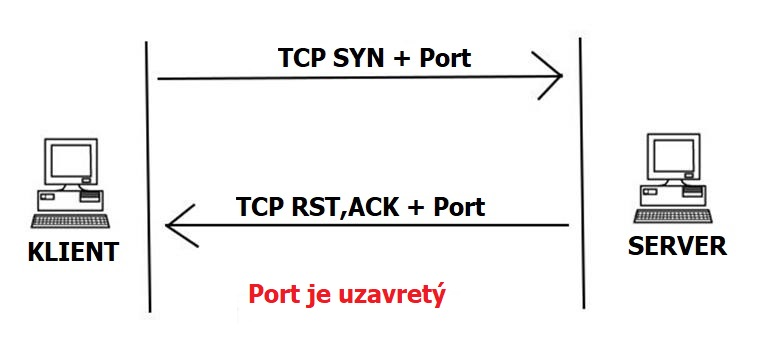
\includegraphics[width=0.375\paperwidth]{obrazky-figures/tcp-closed.jpg}
		\caption{Komunikácia pri zatvorenom porte}
		\label{fig:tcp-clos}
	\end{subfigure}%
	\begin{subfigure}{.5\textwidth}
		\centering
		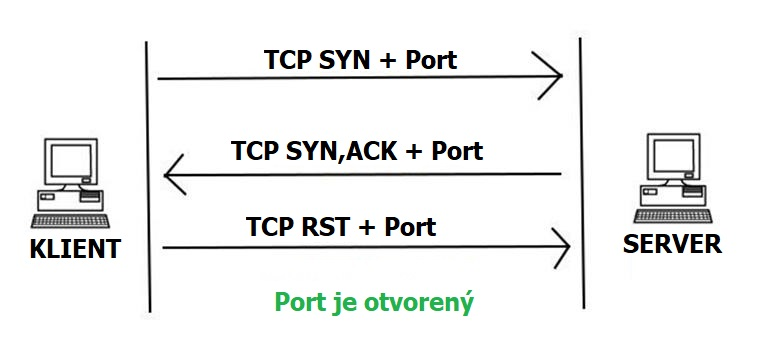
\includegraphics[width=0.375\paperwidth]{obrazky-figures/tcp-open.jpg}
		\caption{Komunikácia pri otvorenom porte}
		\label{fig:tcp-open}
	\end{subfigure}
	\caption{Priebeh komunikácie medzi serverom a klientom pri TCP skenovaní}
	\label{fig:tcp}
\end{figure}


\section{UDP sken}
UDP sken je nespoľahlivý a v~celku nepresný, ak je aktívne blokovanie ICMP správ, na ktorých je založený. Princíp odosielania UDP paketu je veľmi podobný TCP, s~pár zmenami. Soket je vytvorený ako \texttt{RAW UDP} a žiaden kontrolný príznak sa nenastavuje, nakoľko UDP toto nastavenie nepodporuje a nepotrebuje. 

Prázdny UDP paket je odoslaný na požadovaný port a adresu zariadenia v~sieti, ak je to možné a sú dostupné systémové zdroje a vyrovnávacia pamäť.

Pri príjmaní odpovede na tento paket sa vytvorí v novom vlákne \texttt{RAW ICMP} neblokujúci soket a funkcia sa pokúša prijať dáta v~nekonečnom cykle. Pokiaľ \texttt{recv()} zachytí paket, je opäť využitá aritmetika ukazateľov na rozdelenie hlavičiek, ktoré sú uložené v~poradí IP, ICMP, IP a UDP. 

\lstinputlisting[frame=single,numbers=left, language=C++,firstline=207, lastline=210, caption={Aritmetika ukazateľov nad hlavičkami protokolov}]{../src/isamon.cpp}

Tieto operácie sú prevedené na základe referencie\footnote{https://stackoverflow.com/questions/47042355/access-udp-from-icmp-message} a sú nutné na to, aby bolo možné v~jednom pakete prijať ICMP aj UDP odpoveď naraz a tak určiť kto nám odpovedal a na aký port bola táto správa určená. Ak zachytíme ICMP typu \texttt{ICMP\_UNREACH} a kódu \texttt{ICMP\_UNREACH\_PORT} uložíme adresu z~UDP odpovede do vektoru blokovaných portov. Po skončení príjmanie priterujeme cez všetky porty a vypíšeme všetky, ktoré sa nenechádzajú vo vektore blokovaných portov.

\begin{figure}[H]
	\centering
	\begin{subfigure}{.5\textwidth}
		\centering
		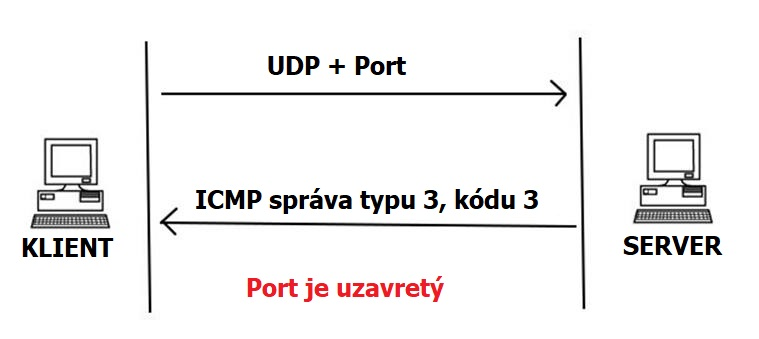
\includegraphics[width=0.375\paperwidth]{obrazky-figures/udp-closed.jpg}
		\caption{Komunikácia pri zatvorenom porte}
		\label{fig:udp-clos}
	\end{subfigure}%
	\begin{subfigure}{.5\textwidth}
		\centering
		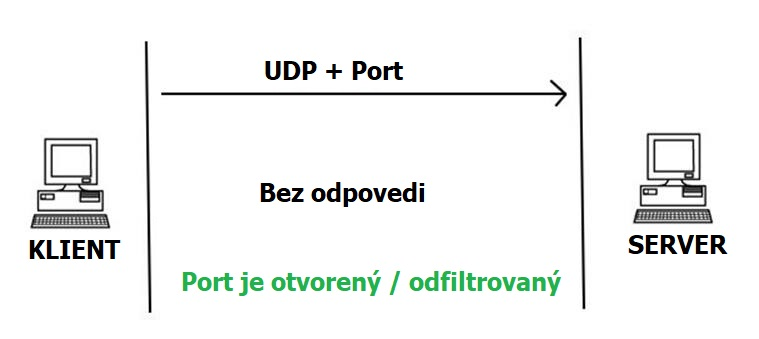
\includegraphics[width=0.375\paperwidth]{obrazky-figures/udp-open.jpg}
		\caption{Komunikácia pri otvorenom porte}
		\label{fig:udp-open}
	\end{subfigure}
	\caption{Priebeh komunikácie medzi serverom a klientom pri UDP skenovaní}
	\label{fig:udp}
\end{figure}


\chapter{Použitie}
Nastavenia a spúšťania programu: 

\texttt{isamon [-h] [-i <interface>] [-t] [-u] [-p <port>] [-w <ms>] -n <net\_address/mask> }

Kde prepínače znamenajú nasledovné: 

\texttt{\hspace{5mm}-h \hspace{5mm}-{}-help \hspace{3mm}}- zobrazí nápovedu

\texttt{\hspace{5mm}-i \hspace{5mm}-{}-interface <interface> \hspace{3mm}}- rozhranie na ktorom bude zariadenie skenovať

\texttt{\hspace{5mm}-n \hspace{5mm}-{}-network <net\_address/mask> \hspace{3mm}} - IP adresa s~maskou siete na skenovanie

\texttt{\hspace{5mm}-t \hspace{5mm}-{}-tcp \hspace{3mm}} - použije TCP

\texttt{\hspace{5mm}-u \hspace{5mm}-{}-udp \hspace{3mm}} - použije UDP

\texttt{\hspace{5mm}-p \hspace{5mm}-{}-port <port>\hspace{3mm}} - špecifikácia skenovaného portu, inak celý rozsah

\texttt{\hspace{5mm}-w \hspace{5mm}-{}-wait <ms>\hspace{3mm}} - maximálne prípustné RTT

\section{Chybové hlášky}
Kódy, s~ktorými sa program môže ukončiť pri chybe sú rôzne na základe funkcií a problémov, ktoré chybu vyvolali.

\texttt{0 = ERR\_HELP} - nesprávna špecifikácia argumentov

\texttt{1 = ERR\_PORT} - nesprávne zadaný port, mimo rozsah

\texttt{2 = ERR\_WAIT} - nesprávne zadaný  časový údaj RTT

\texttt{3 = ERR\_DUPL} - duplicita argumentov

\texttt{4 = ERR\_NETW} - zadaná sieť nieje validná

\texttt{5 = ERR\_SOPT} - zlyhala funkcia setsockopt

\texttt{6 = ERR\_SOCK} - zlyhala funkcia socket

\texttt{7 = ERR\_GAIN} - zlyhala funkcia getifaddrs

\texttt{8 = ERR\_SEND} - zlyhala funkcia sendto

\texttt{9 = ERR\_IOCTL} - zlyhala funkcia ioctl

\texttt{10 = ERR\_RECV} - zlyhala funkcia recv alebo recvfrom

\newpage
\section{Príklady použitia a výstupu}


\hspace{6mm}\texttt{isamon -n 192.168.0.0/24} - prevedie sken siete a zobrazí aktívne zariadenia

\texttt{isamon -n 192.168.0.0/24 -t} - prevedie sken siete, zobrazí aktívne zariadenia a ich otvorené TCP porty

\texttt{isamon -n 192.168.0.0/30 -i eth0} - prevedie sken siete za použitia rozhrania eth0

\texttt{isamon -n 192.168.0.0/28 -t -u -w 10} - prevedie sken siete a a zobrazí aktívne zariadenia s~ich otvorenými TCP a UDP portami s~maximálnych prípustným RTT

\texttt{isamon -n 192.168.0.0/30 -t -p 80} - prevedie sken siete a vypíše aktívne zariadenia a či majú otvorený TCP port 80

\vspace{10mm}

Príklad výstupu: 

\texttt{192.168.1.1} - aktívny klient

\texttt{192.168.1.1 TCP 80} - otvorený TCP port 80

\texttt{192.168.1.1 TCP 22} - otvorený TCP port 20

\texttt{192.168.1.1 UDP 53} - otvorený UDP port 53


\chapter{Záver}
Program sa dá úspešne použiť na zistenie aktívnych klientov v~sieti a ich otvorené porty pre protokol TCP alebo UDP. Aplikácia je limitovaná veľkosťou vyrovnávacej pamäti a nastaveniami jadra na spracovávanie paketov. 

Testovanie prebehlo úspešne na systémoch Linux, za použitia lokálneho stroja Ubuntu 17.04 a virtuálneho stroja CentOS 7 s~využitím vagrantu.

Pri programovaní tejto aplikácie som sa naučil lepšie pracovať s~druhou až štvrtou vrstvou ISO OSI modelu a pochopil princípom skenovania siete a portov.

%=========================================================================
